\documentclass[12pt]{article}

\usepackage[english]{babel}
\usepackage[utf8]{inputenc}
\usepackage[top=2cm, left=2cm, right=2cm, bottom=2cm]{geometry}
\usepackage[document]{ragged2e}
\usepackage{tikz,minted,times}

\setlength\parindent{0pt}
\sloppy
\usetikzlibrary{automata,positioning,arrows}
\tikzset{node distance=2.5cm,every state/.style={semithick,fill=gray!10},initial text={},double distance=2pt,every edge/.style={draw,->,>=stealth,auto,semithick}}
\usemintedstyle{colorful}

\title{COMP SCI 7411 Event Driven Computing Practice 1 Plan}
\author{Tinson Lai \\ a1812422}
\date{\today}

\begin{document}

\maketitle

\section{Locking}

\begin{figure}[H]
  \centering
  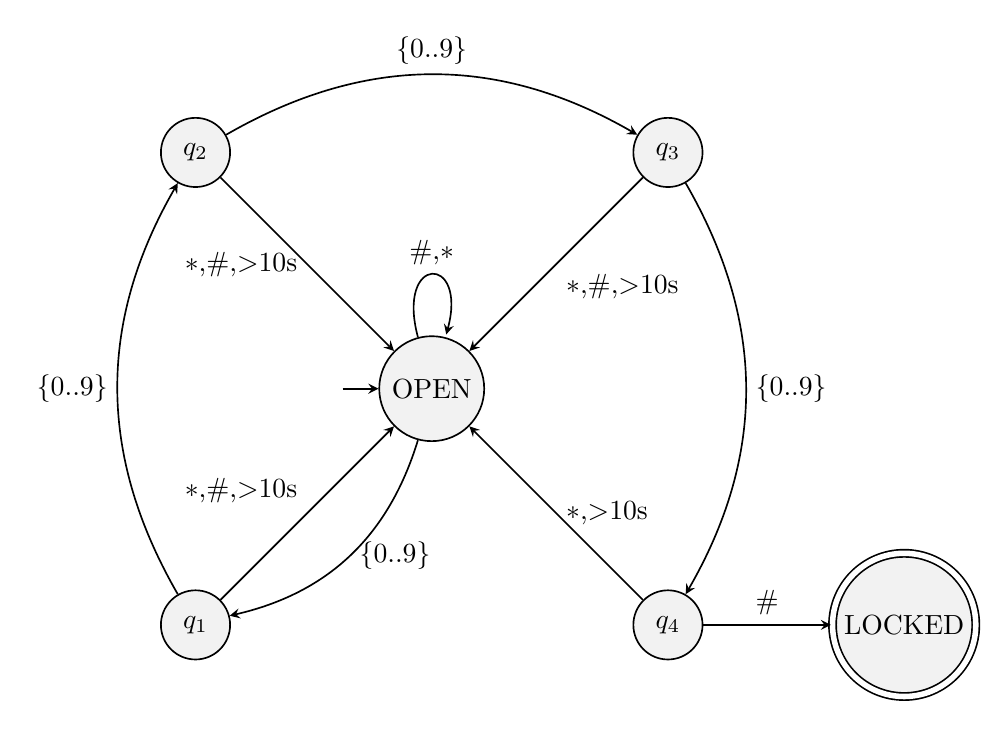
\begin{tikzpicture}
    \node[state, initial] at (3, 3) (open){OPEN};
    \node[state] at (0, 0) (q1){$q_1$};
    \node[state] at (0, 6) (q2){$q_2$};
    \node[state] at (6, 6) (q3){$q_3$};
    \node[state] at (6, 0) (q4){$q_4$};
    \node[state, accepting] at (9, 0) (locked){LOCKED};

    \draw

    (open) edge[loop above] node{$\#$,$*$} (open)
    (open) edge[bend left, right] node{$\left\{0..9\right\}$} (q1)
    (q1) edge[bend left, left] node{$\left\{0..9\right\}$} (q2)
    (q2) edge[bend left, above] node{$\left\{0..9\right\}$} (q3)
    (q3) edge[bend left, right] node{$\left\{0..9\right\}$} (q4)

    (q1) edge node{$*$,$\#$,$>$10s} (open)
    (q2) edge[left] node{$*$,$\#$,$>$10s} (open)
    (q3) edge node{$*$,$\#$,$>$10s} (open)
    (q4) edge node{$\#$} (locked)
    (q4) edge[right] node{$*$,$>$10s} (open)

    ;
  \end{tikzpicture}
  \caption{Locking Process}
  \label{fig:locking}
\end{figure}

\section{Unlocking}

\begin{figure}[H]
  \centering
  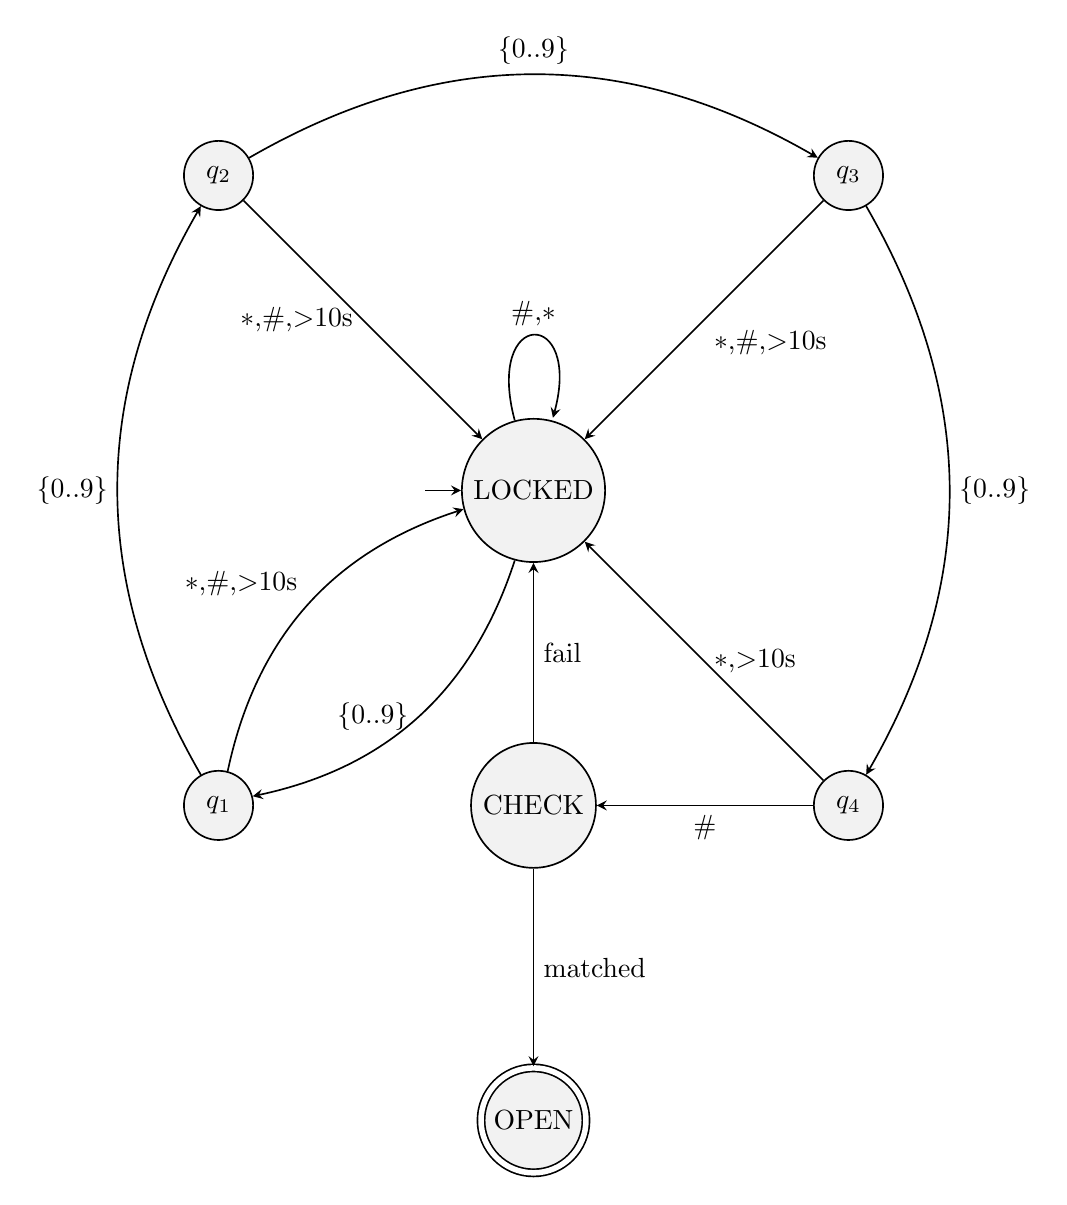
\begin{tikzpicture}
    \node[state, initial] at (4, 8) (locked){LOCKED};
    \node[state] at (0, 4) (q1){$q_1$};
    \node[state] at (0, 12) (q2){$q_2$};
    \node[state] at (8, 12) (q3){$q_3$};
    \node[state] at (8, 4) (q4){$q_4$};
    \node[state] at (4, 4) (check){CHECK};
    \node[state, accepting] at (4, 0) (open){OPEN};

    \draw

    (locked) edge[loop above] node{$\#$,$*$} (locked)
    (locked) edge[bend left, left] node{$\left\{0..9\right\}$} (q1)
    (q1) edge[bend left, left] node{$\left\{0..9\right\}$} (q2)
    (q2) edge[bend left, above] node{$\left\{0..9\right\}$} (q3)
    (q3) edge[bend left, right] node{$\left\{0..9\right\}$} (q4)

    (q1) edge[bend left] node{$*$,$\#$,$>$10s} (locked)
    (q2) edge[left] node{$*$,$\#$,$>$10s} (locked)
    (q3) edge node{$*$,$\#$,$>$10s} (locked)
    (q4) edge node{$\#$} (check)
    (q4) edge[right] node{$*$,$>$10s} (locked)

    (check) edge[right] node{fail} (locked)
    (check) edge node{matched} (open)

    ;
  \end{tikzpicture}
  \caption{Unlocking Process}
  \label{fig:unlocking}
\end{figure}

\section{Notations}

The designs above have several notations:
\begin{itemize}
  \item Intermediate states within the digits entering process are named $q_i$ where $i$ represents the number of digits shown in the panel display.
  \item $\#$ means presssing the key $\#$ once, similar for $*$. $\left\{0..9\right\}$ means pressing one of the numeric keys on the panel once.
  \item $q_1$ will also starts a timer.
  \item $q_4$ will lock all numeric keys so there are only two possible inputs ($*$ and $\#$).
  \item The CHECK state in Figure \ref{fig:unlocking} is a special intermediate state which are not visually presented to the user. It just depicts a state where the system has to check for password correctness.
  \item "$>$10s" means the timer has recorded a duration longer than 10 seconds. An alert will be delivered to the user and the input will be cleared as required.
\end{itemize}

\section{Timer}

The timer started in state $q_1$ in Figure \ref{fig:locking} and \ref{fig:unlocking} can be interrupted by $*$ or $\#$ as described previously. Any subsequent inputs of digits following the first digit will not affect the status of the timer. Thus the diagram will be as simple as Figure \ref{fig:timer}.

\begin{figure}[H]
  \centering
  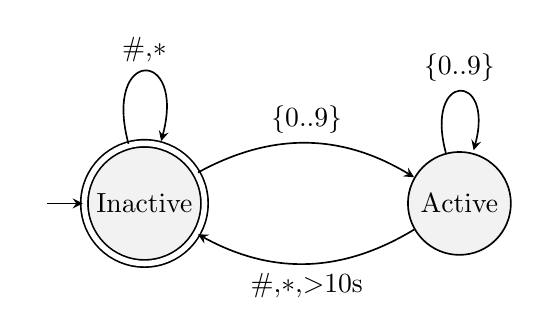
\begin{tikzpicture}
    \node[state, initial, accepting] at (0, 0) (inactive){Inactive};
    \node[state] at (4, 0) (active){Active};

    \draw

    (inactive) edge[loop above] node{$\#$,$*$} (inactive)
    (inactive) edge[bend left] node{$\left\{0..9\right\}$} (active)
    (active) edge[loop above] node{$\left\{0..9\right\}$} (active)
    (active) edge[bend left] node{$\#$,$*$,$>$10s} (inactive)

    ;
  \end{tikzpicture}
  \caption{Timer}
  \label{fig:timer}
\end{figure}

\section{Disabling Numeric Keys}

Another design choice is disabling numeric keys in the panel when $q_4$ is reached.

\begin{figure}[H]
  \centering
  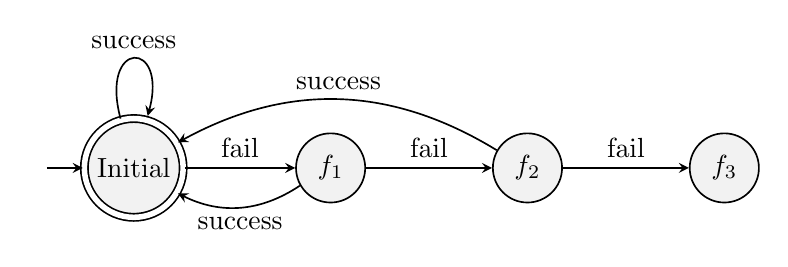
\begin{tikzpicture}
    \node[state, initial, accepting] (initial){Initial};
    \node[state, right of=initial] (f1){$f_1$};
    \node[state, right of=f1] (f2){$f_2$};
    \node[state, right of=f2] (f3){$f_3$};

    \draw

    (initial) edge node{fail} (f1)
    (f1) edge node{fail} (f2)
    (f2) edge node{fail} (f3)

    (initial) edge[loop above] node{success} (initial)
    (f1) edge[bend left, below] node{success} (initial)
    (f2) edge[bend right, above] node{success} (initial)

    ;
  \end{tikzpicture}
  \caption{Numeric Keys Disabling}
  \label{fig:disable}
\end{figure}

A permanent lock will also be applied if the user fails to enter the correct password three times and it's not possible to input digits anymore, and this is show as the state $f_3$ in Figure \ref{fig:disable}.

\section{Notes}

Although $\#$ and $*$ seem to have identical behaviour in the state diagram in the state diagram, in the actual implementation, I tried to display different alerts to the user if they press $\#$ without an appropriate input. For example, an alert warning the user about incorrect password etc.

\end{document}
